
\section{\lsystem types}
\label{sec:lsysTypes}

In this section we will describe different types of \lsystems.
Some types may require an extension of described formal definition of \lsystem but it will be omitted.

\lsystems described so far are called \emph{deterministic \lsystems} because their rewriting system is deterministic.
\emph{Bracketed \lsystems} allow to save and load a state of the interpretation.
This can be used to model branches of plants more easily.
\emph{Stochastic \lsystems} can randomize result model to suppress its artificiality.
\emph{Context-sensitive \lsystems} allows to rewrite symbol depending on its context (symbols around it).
Symbols in \emph{parametric \lsystems} can hold any number of arguments which can be used while rewriting or interpreting symbols.

Any of described types can be combined together.



\subsection{Deterministic \lsystems}

\newcommand{\dzerolsystem}{\mbox{D0L-system}\xspace}
\newcommand{\dlsystem}{\mbox{dL-system}\xspace}


\begin{wrapfigure}{r}{0.50\textwidth}
	\vspace{-30pt}
	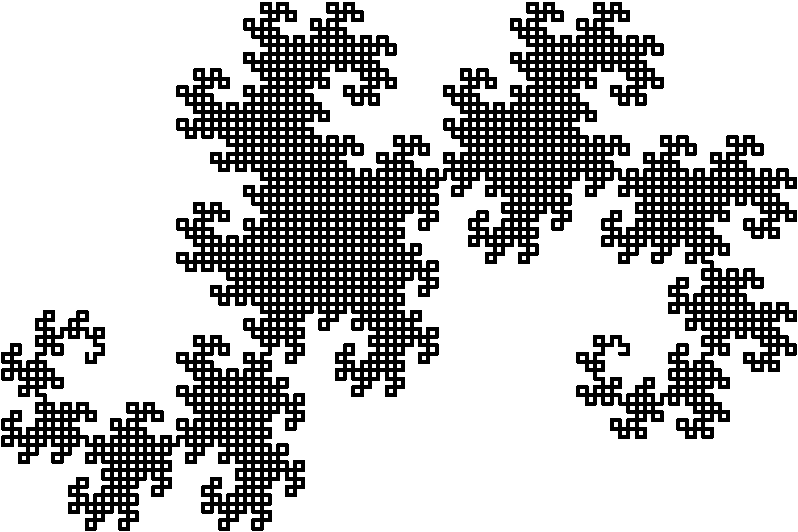
\includegraphics[width=\linewidth]{BasicLsystem}
	\caption{Dragon curve}
	\label{fig:basicLsystem}
\end{wrapfigure}


Basic \lsystem type described by previous formal definition is called \dzerolsystem\footnote{\dzerolsystem is also called just \dlsystem~\cite{Zar04}.}.
\emph{D} means that rewriting is deterministic and \emph{0} means it is context-free.
The result of \dzerolsystem depends only on the initial string of symbols.

This type of \lsystem is often used to generate fractal curves.
With \dzerolsystem in \autoref{fig:basicLsystem} we can generate Dragon curve that you can see in \autoref{lsys:basicLsystemSrc}.

\begin{Lsystem}[label=lsys:basicLsystemSrc,caption={\dzerolsystem for generation of Dragon curve (\autoref{fig:basicLsystem})}]
lsystem DragonCurve {
	set iterations = 12;
	set symbols axiom = L;
	interpret R L as DrawForward(5);
	interpret + as TurnLeft(90);
	interpret - as TurnLeft(-90);
	rewrite L to L + R +;
	rewrite R to - L - R;
}
process all with SvgRenderer;
\end{Lsystem}


\subsection{Bracketed \lsystems}

First and important extension to \dzerolsystem is branching system.
This type of \lsystem is called Bracketed \lsystem\cite{PL91}.
Branching is so fundamental feature that Bracketed \lsystems are often called just \lsystems.

%!!!!!!!!!!!!!!!!!!!!!!!!!!!!!
Branching system extends symbol interpretation by two commands \emph{start branch} and \emph{end branch}.
These commands are nearly always represented as symbols of brackets (from which bracketed \lsystems got their name).
Open bracket "$[$" as a start branch and close bracket "$]$" as close branch.

Start branch command saves the state of interpretation which can be loaded by end branch command later.
In turtle graphics interpretation state is position, orientation and drawing color of turtle.
More than one states can be saved at the same time, last saved state will be loaded first.
This behavior is natural and could be compared to a pairing of brackets.

Branching extends linear string of symbols to a tree structure.
Individual branches do not affect each other nor their root.
This allows to model plants more easily and create more complex models.

Bracketed \lsystem in \autoref{lsys:branchingSrc} demonstrates usage of branching system to produce plant-like model which you can see in \autoref{fig:branching}.
Note that color of segments indicates their type and age.
Black segments are drawn with symbol $F$ and they represent segments from previous iteration.
Green segments are drawn with symbol $A$ and they are new compared to the previous iteration.

\begin{Lsystem}[label=lsys:branchingSrc,caption={Bracketed \lsystem which creates plant-like model (\autoref{fig:branching})}]
lsystem PythagorasTree {
	set symbols axiom = A;
	set initialAngle = 90;
	set iterations = 4;	
	interpret A F as DrawForward(16);
	interpret + as TurnLeft(45);
	interpret - as TurnLeft(-45);
	@interpret [ as StartBranch;@
	@interpret ] as EndBranch;@
	rewrite A to F [ + A ] [ - A ] F A;
	rewrite F to F F;
}
process all with SvgRenderer;
\end{Lsystem}

\begin{figure}[h]
	\centering
	\subfloat{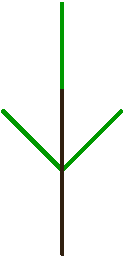
\includegraphics[scale=1]{Branching1}} ~
	\subfloat{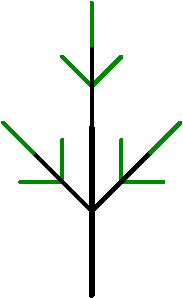
\includegraphics[scale=1]{Branching2}} ~
	\subfloat{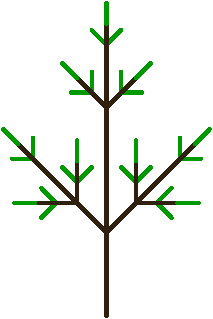
\includegraphics[scale=1]{Branching3}} ~
	\subfloat{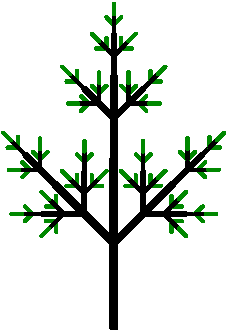
\includegraphics[scale=1]{Branching4}}
	\caption{First four iterations of bracketed \lsystem in \autoref{lsys:branchingSrc}}
	\label{fig:branching}
\end{figure}



\subsection{Stochastic \lsystems}

\newcommand{\zerolsystem}{\mbox{0L-system}\xspace}
\newcommand{\zerolsystems}{\mbox{0L-systems}\xspace}

All plants generated by same deterministic \lsystem are identical.
Forest made by trees which are identical looks artificial and can not be used in films or video games.
Stochastic \lsystems solve this problem because they can produce randomized model.
Stochastic \lsystems are called \zerolsystem where 0 means they are context-free.

% kde se vzal modle!!!!!!!!!!!!!!!!!!!!!!!!

Randomization of a model produced by stochastic \lsystem can be done in two places, in rewrite rules or in the interpretation of symbols (or in both).
Randomization in interpretation can only change properties of interpreted symbols such as lengths of lines or turning angles, the topology of the model remains unchanged.
In contrast with rewrite rule randomization which can also change topology of the model.
Rewrite rule randomization is done by defining more replacements for one rewrite rule.
Rewriting system will pick random replacement if rewrite rule is applied.
Each replacement can have different probability to be picked.

In \autoref{fig:randComparison} are shown 3 models of plant generated by stochastic \lsystems.
The first image (\ref{fig:randComparisonNo}) was generated without any randomization.
The second image (\ref{fig:randComparisonInt}) was generated with interpretation randomization of line lengths and angles.
For the last image (\ref{fig:randComparisonBoth}) was also added topology randomization with rewrite rule randomization (\autoref{lsys:randExample}).

\begin{figure}[h]
	\centering
	\subfloat[No randomization]{
		\label{fig:randComparisonNo}
		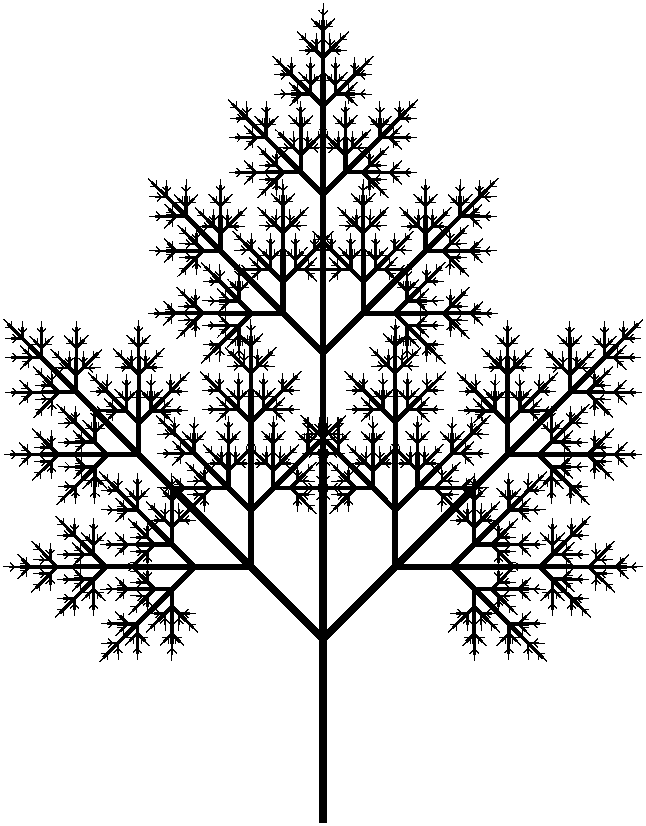
\includegraphics[width=0.3\textwidth]{StochasticLsystemExample-NoStochasism}
	} ~
	\subfloat[Angles, lengths randomized]{
		\label{fig:randComparisonInt}
		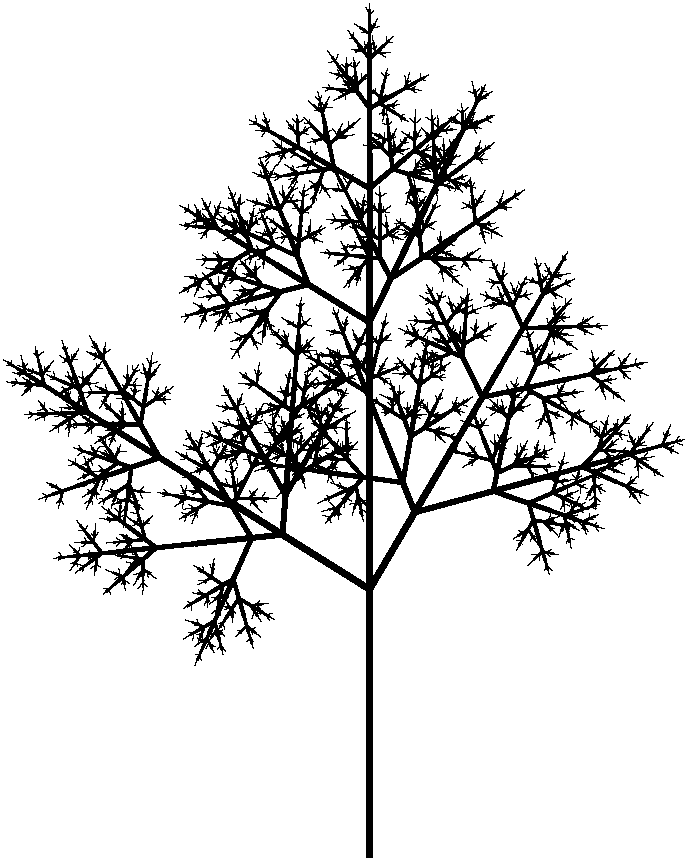
\includegraphics[width=0.32\textwidth]{StochasticLsystemExample-InterpretationStochasism}
	} ~
	\subfloat[Also topology randomized]{
		~
		\label{fig:randComparisonBoth}
		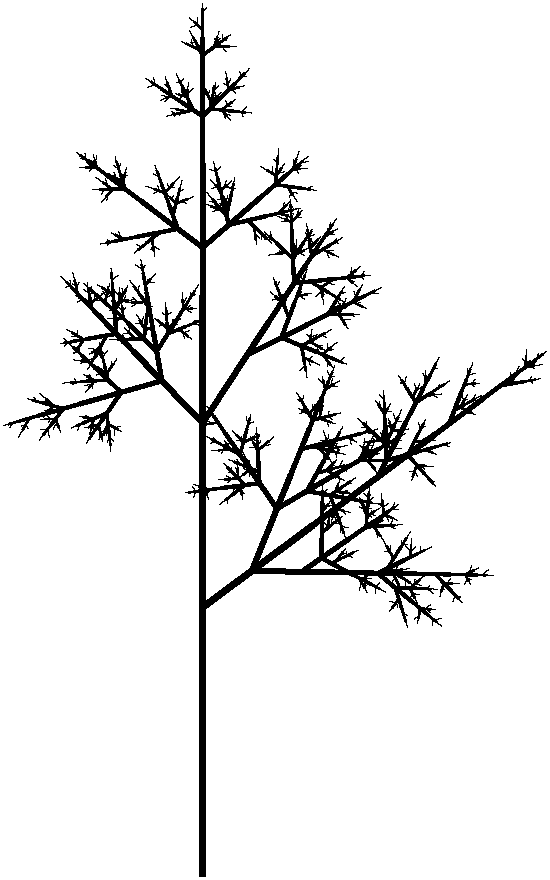
\includegraphics[width=0.25\textwidth]{StochasticLsystemExample-BothStochasism}
		~
	}
	\caption{Comparison between non-randomized and randomized plant model}
	\label{fig:randComparison}
\end{figure}

\begin{Lsystem}[label=lsys:randExample,caption={Stochastic \lsystem with randomized interpretation of symbols and rewrite rule replacements}]
lsystem StochasticLsystemExample {
	set symbols axiom = X;
	set iterations = 8;
	set initialAngle = 90;
	interpret F(age) as DrawForward(@1.8^age*random(0.5,1.5)@, age/2);
	interpret + as TurnLeft(@45 + random(-20, 20)@);
	interpret - as TurnLeft(@-45 + random(-20, 20)@);
	interpret [ as StartBranch;
	interpret ] as EndBranch;
	rewrite F(age) to F(age + 1);
	@rewrite X@
		@to F(1) [ + X ] [ - X ] F(1) X  weight 4 or@
		@to F(1) [ + X ]         F(1) X  weight 1 or@
		@to F(1)         [ - X ] F(1) X  weight 1;@
}
process all with SvgRenderer;
\end{Lsystem}


\subsection{Context-sensitive \lsystems}

\newcommand{\onelsystems}{\mbox{1L-systems}\xspace}
\newcommand{\twolsystems}{\mbox{2L-systems}\xspace}

Rewriting of symbols in \zerolsystems is context-free, rewrite rules are applied on the symbols regardless of their context (symbols around it).
However rewriting of a symbol can also depend on its context.
This is useful in simulating the flow of signals (nutrients or hormones) in plant model~\citep{PL91}.

Formally there are two types of context-sensitive L-systems, \onelsystems and \twolsystems.
Rewrite rules of \onelsystems checks context only on one side (left or right) whereas rewrite rules of \twolsystems checks context on both sides.
Since \onelsystems are just \twolsystems with one context empty we will consider context-sensitive \lsystems as \twolsystems.

Context-sensitive \lsystem in \autoref{lsys:signalPropagarionSrc} shows simulation of signal propagation in the string of symbols.
Result is in \autoref{fig:signalPropagarion}.

\begin{Lsystem}[label=lsys:signalPropagarionSrc,caption={Context-sensitive \lsystems simulating signal propagation}]
lsystem RewritingExample {
	set symbols axiom = B A A A A A;
	set iterations = 6;
	set interpretEveryIteration = true;
	@rewrite {B} A     to B;@
	@rewrite     B {A} to A;@
}
process all with SymbolPrinter;
\end{Lsystem}

\begin{table}[h]
	\centering
	\begin{tabular}{c l}
   		\toprule
   		Iteration & String of symbols \\
   		\midrule
		0 & B A A A A A \\
		1 & A B A A A A \\
		2 & A A B A A A \\
		3 & A A A B A A \\
		4 & A A A A B A \\
		5 & A A A A A B \\
		6 & A A A A A A \\
		\bottomrule
	\end{tabular}
	\caption{Axiom and first 6 iterations of \lsystem in \autoref{lsys:signalPropagarionSrc} showing signal propagation in the string of symbols}
	\label{fig:signalPropagarion}
\end{table}


\subsubsection{Context-sensitive bracketed \lsystems}
\label{sec:bracketedLsystems}

If we add context-sensitive rewrite rule to bracketed \lsystems the situation will be more difficult.
The context matching procedure must take into account the branches.
Following rules define natural behavior of context between branches:
\begin{enumerate*}
	\item \label{enum:ctxRule1} two symbols are neighbors even if there are some branches between them,
	\item \label{enum:ctxRule2} left neighbor of the first symbol in branch is symbol before branch,
	\item \label{enum:ctxRule3} the last symbol in a branch does not have a right neighbor,
	\item \label{enum:ctxRule4} unmatched symbols at the end of a branch are ignored,
	\item \label{enum:ctxRule5} the order of branches is insignificant.
\end{enumerate*}

% co to je context matching !!!!!!!!!!!!!!!!!!!!!!!!!!!!!
\autoref{tbl:bracketCtxt} shows examples of context-matching in bracketed \lsystems with references to according rules.

\begin{table}[h]
	\centering
	\begin{tabular}{c c c p{128pt} c c}
   		\toprule
   		Left ctx. & Symbol & Right ctx. & Symbol string & Match & Rule\\
   		\midrule
		 & X & Y & A B {\btHL X} [ A [ B ] ] [ C ] {\btHL Y} & yes & \ref{enum:ctxRule1} \\
		 & X & Y & A B X [ Y B ] C Y & no &  \\
		 Y & X & & A B {\btHL Y [ X} A B ] C & yes & \ref{enum:ctxRule2} \\
		 Y & X & & A B {\btHL Y [ [ X} A ] B ] C & yes & \ref{enum:ctxRule2} \\
		 & X & Y & A [ B X ] Y & no & \ref{enum:ctxRule3} \\
		 & X & [ Y ] & A B {\btHL X [ Y} A B ] A  & yes & \ref{enum:ctxRule4} \\
		 & X & [ [ Y ] ] & A B {\btHL X [ [ Y} A B ] C ] & yes & \ref{enum:ctxRule4} \\
		 & X & [ Y ] & A B {\btHL X} [ A B ] {\btHL{}[ Y} ] A  & yes & \ref{enum:ctxRule5} \\
		 & X & [ Y ] [ Z ] & A B {\btHL X [ Z} ] {\btHL{}[ Y} ] A  & yes & \ref{enum:ctxRule5} \\
		\bottomrule
	\end{tabular}
	\caption{Examples of context matching in bracketed \lsystems}
	\label{tbl:bracketCtxt}
\end{table}

Context in bracketed \lsystems can be used for propagation of signals through tree structure.
There are two basic types of signals.
First is \emph{acropetal} signal which spreads from root to branches and second is \emph{basipetal} which spreads in other way i.e. from branches to root.
This can be used well in plant modeling.

\autoref{fig:signalPropagation} shows simulation of acropetal (\ref{fig:acropetalSignal}) and basipetal (\ref{fig:basipetalSignal}) signals in static plant-like structure.
Each figure shows first 5 iterations and segments with the signal are marked as bolder line.
\lsystem in \autoref{lsys:signalPropagation} simulates acropetal signal propagation and its result is in \autoref{fig:acropetalSignal} (image) and \autoref{fig:signalPropagationTable} (symbols).

% označit zem !!!!!!!!!!
\begin{figure}[h!]
	\centering
	\subfloat[Acropetal signal propagation]{
		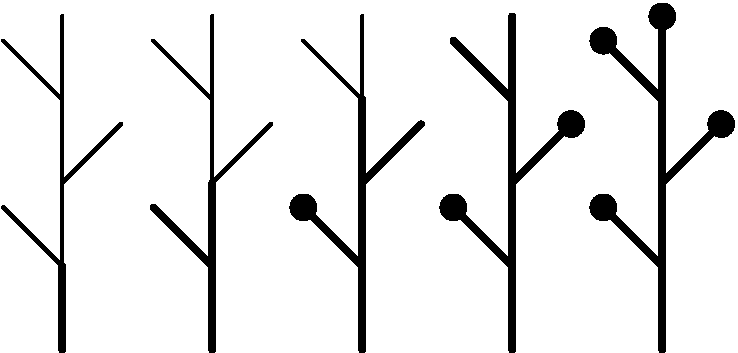
\includegraphics[scale=0.55]{AcropetalSignal}
		\label{fig:acropetalSignal}
	}
	\hspace{2mm}
	\subfloat[Basipetal signal propagation]{
		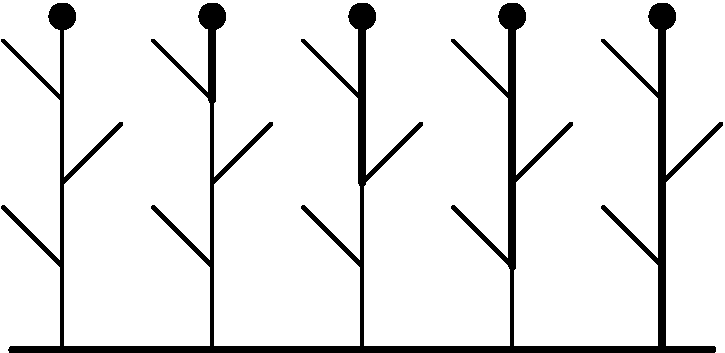
\includegraphics[scale=0.55]{BasipetalSignal}
		\label{fig:basipetalSignal}
	}
	\caption{Signal propagation simulated with context-sensitive bracketed \lsystems}
	\label{fig:signalPropagation}
\end{figure}

\begin{Lsystem}[label=lsys:signalPropagation,caption={\lsystem simulating acropetal signal propagation (\autoref{fig:acropetalSignal})}]
lsystem AcropetalSignal extends Branches {
	set symbols axiom = B [ + A ] A [ - A ] A [ + A ] A;
	// ignore + and - symbols in context search
	@set symbols contextIgnore = + -;@
	set iterations = 3;
	// interpret every iteration to see signal propagation
	set interpretEveryIteration = true;
	set initialAngle = 90;
	interpret A as DrawForward(50, 2);
	interpret B as DrawForward(50, 4);
	interpret + as TurnLeft(45);
	interpret - as TurnLeft(-45);
	@rewrite { B } A to B;@
}
process all with SvgRenderer;
\end{Lsystem}


\begin{table}[h]
	\centering
	\begin{tabular}{c c}
   		\toprule
   		Iteration & String of symbols \\
   		\midrule
		0 & B [ + A ] A [ - A ] A [ + A ] A \\
		1 & B [ + B ] B [ - A ] A [ + A ] A \\
		2 & B [ + B ] B [ - B ] B [ + A ] A \\
		3 & B [ + B ] B [ - B ] B [ + B ] B \\
		\bottomrule
	\end{tabular}
	\caption{Result of \lsystem simulating acropetal signal propagation in \autoref{lsys:signalPropagation}}
	\label{fig:signalPropagationTable}
\end{table}


\subsection{Parametric \lsystems}

Symbols in parametric \lsystems can hold any number of arguments.
Arguments are often floating point numbers but they can be more complicated structures.
Arguments can be used in interpretation definition to send values like color or length of line to an interpretation routine.
Arguments can be also used in rewrite rules to determine whether rewrite symbol or not and to determine new arguments for rewritten symbols.
In context \twolsystems is also possible to get arguments from symbols in context and use them in rewrite rules.

\lsystem in \autoref{fig:scParams} shows usage of parameters of symbols in interpretation methods and in rewrite rules along with the result.


\newsavebox{\lstBox}
\begin{lrbox}{\lstBox}
\begin{Lsystem50}
lsystem Circles {
	set symbols axiom =	[ X ] +
		[ X ] + [ X ] + [ X ];
	set iterations = 7;
	interpret F as MoveForward;
	interpret K as DrawCircle;
	interpret + as @TurnLeft(90)@;
	interpret - as @TurnLeft(-90)@;
	interpret [ as StartBranch;
	interpret ] as EndBranch;
	rewrite @K(n) to K(2*n)@;
	rewrite @F(n) to F(2*n)@;
	rewrite X to @K(2) F(3)@
		[ + X ] [ - X ] X;
}
process all with SvgRenderer;
\end{Lsystem50}
\end{lrbox}

\begin{figure}[h!]
	\subfloat{
		\usebox{\lstBox}
	} \hfill
	\subfloat{
		\minipage{0.47\linewidth}\noindent
		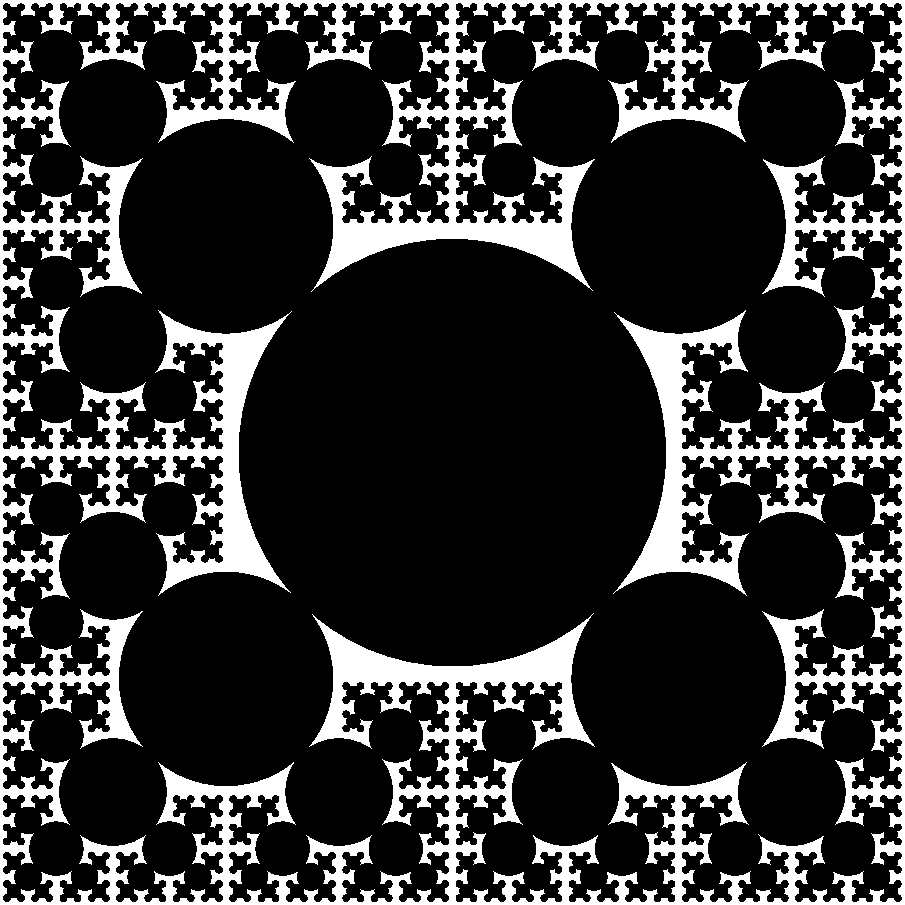
\includegraphics[width=\textwidth]{Circles}
		\endminipage
	}
	\caption{Parameters usage in \lsystem interpretation methods and in rewrite rules along with the result}
	\label{fig:scParams}
\end{figure}

In \autoref{fig:redEndPythagoras} is more complicated model, the Pythagoras tree.
It is named by Pythagoras because if we denote length of edge of the base square as $c$ and length of edges of squares raised from the base square as $a$ and $b$ Pythagorean theorem describes theirs relation as $c^2 = a^2 + b^2$.
This formula also says that area of the base square is equal to sum of areas of its child squares.
The relation applies to all squares in the tree.

\begin{figure}[H]
	\centering
	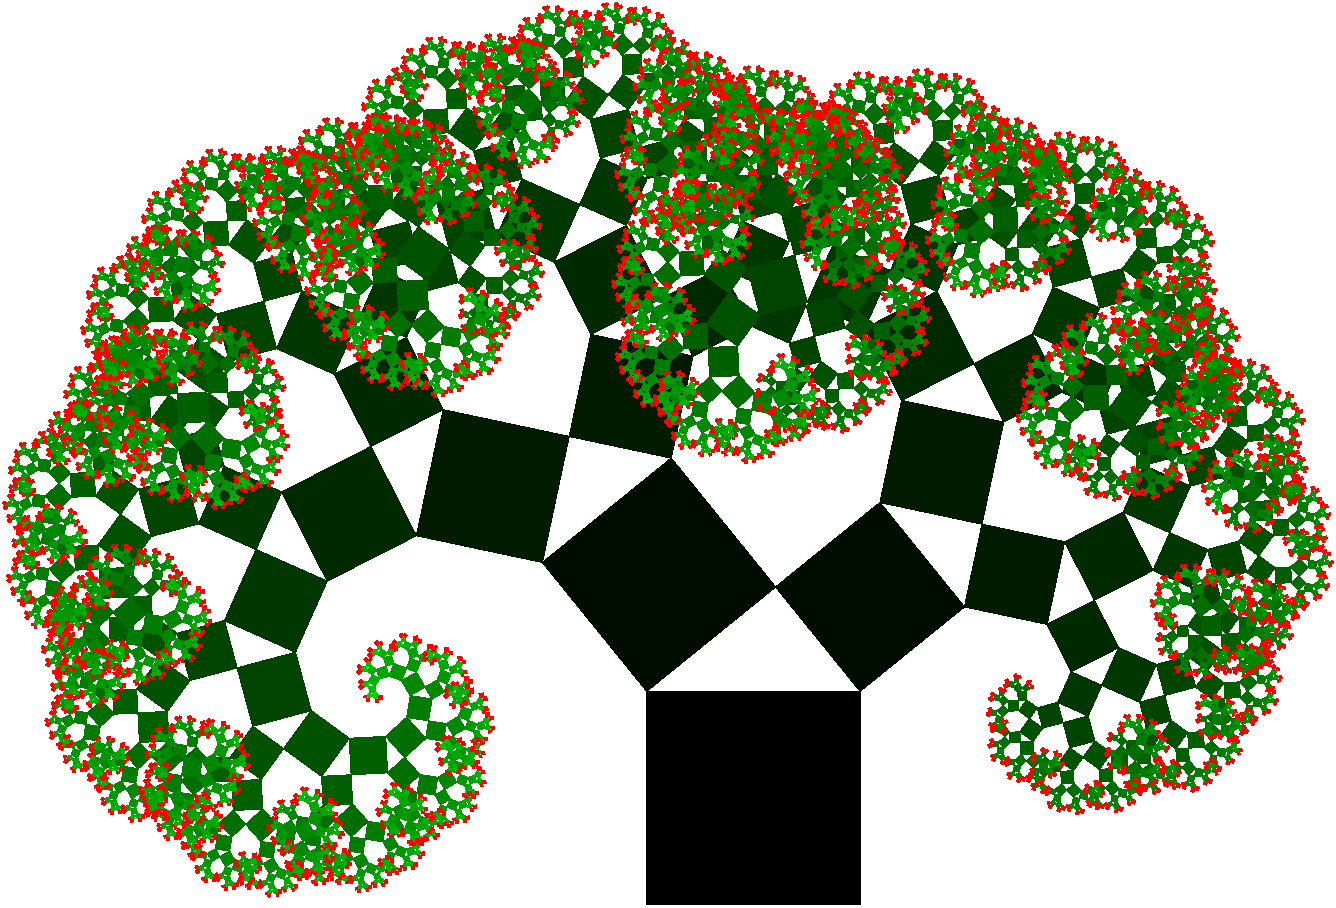
\includegraphics[width=0.95\linewidth]{PythagorasTree2dRedEnd}
	\caption{Pythagoras tree created with parametric \lsystem}
	\label{fig:redEndPythagoras}
\end{figure}
































